% Instructor's Guide to Euclidean Geometry Notes
\documentclass{tufte-handout}

%\geometry{showframe}% for debugging purposes -- displays the margins

%%%% Packages to make things pretty
\usepackage{amsmath,amsthm}
\usepackage{booktabs}
\usepackage{graphicx}
\setkeys{Gin}{width=\linewidth,totalheight=\textheight,keepaspectratio}
\graphicspath{{graphics/}}
\usepackage{units}
\usepackage{fancyvrb}
\fvset{fontsize=\normalsize}
\usepackage{multicol}
\usepackage{pdfpages}
\usepackage{paralist}

%%%% Theorem Environments
\theoremstyle{definition}
\swapnumbers
\newtheorem{problem}{Problem}[section]
\newtheorem{conjecture}[problem]{Conjecture}
\newtheorem*{definition}{Definition}
\newtheorem*{theorem}{Theorem}
\newtheorem{question}[problem]{Question}
\newtheorem{challenge}[problem]{Challenge}
\newtheorem*{postulate}{Postulate}

%%%%%


\title{Euclidean Geometry}
\author[Instructor's Manual]{Instructor's Manual}
\date{Spring 2016} 

\begin{document}

\maketitle

\begin{marginfigure}
    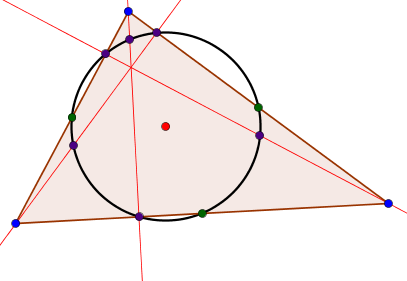
\includegraphics{NPC}
\end{marginfigure}


\setcounter{section}{0}
\setcounter{problem}{0}
\section{Instructor's Preface}

This opening section is a set of notes aimed at an instructor who wishes to use these notes for the first time.
I have deliberately aimed the discussion at someone who is \emph{new} to using inquiry-based methods in class.
More experienced instructors will know what to ignore and adapt things to their own style without much effort.
I hope newcomers to IBL will appreciate specific instructions about how I run a class from these notes.

Below the reader will find discussion of all of the major components of the course, and how I run the critically important first day.
Then I give some contextual notes for each item in the script, section-by-section.

\subsection{General Orientation}

idea of course: situational factors, big idea, main goals. idea of flexibility.\\

general non-sense goes here. philosophical advice. aims of the course. orientation stuff.  replace this later.\\

include Tim McNichol reference and idea

\subsection{Class Materials}

compass and straightedge, dynamic geometry software, Euclid from Green Lion Press, 
research notebook


\subsection{The First Class Meeting}

The importance of a good first meeting cannot be understated.
Students have to reach an understanding of how class will run and what is expected of them.
Also, at least one student has to have very visible success in front of the class.
Here is how I run the first day:\\[.1in]

\begin{compactdesc}
\item[\textbf{Phase I}] I arrive early and put the first three definitions and Conjecture 1.1 on the board.
I reassure students that they don't need to copy this down, as I will hand it out to them later.
I also try to put them at ease with plenty of small talk about how I need to work out between semesters so that I can write so much.
This usually spills into the first minute or two of class.
When I am certain that the class is all present, I introduce myself briefly and ask them to try to prove the statement on the board with a partner.
I tell them that they should just use whatever they think they recall from high school geometry.\\[.1in]

\item[\textbf{Phase II}] Now I give the students time to work in pairs.
As they work, I go take the time to introduce myself to them and learn their names one pair at a time.
Along the way I have to take a couple of questions about mathematics, but mostly I am trying (1) to put faces to names on the roster and (2) to make myself more approachable.\\[.1in]

\item[\textbf{Phase III}] After about twenty five minutes, someone has an argument for at least part of Conjecture 1.1.
I call for volunteers, but if none materialize I call on a pair that I saw do something worthy.
I invite one student to come to the board to share their ideas.
After they get up, but before they start speaking, I interrupt and explain the basic ground rules to the class.\\[.1in]

We use only last names.
We are polite to a fault.
When in our seats, we ask questions rather than give arguments.
The presenter's job is to convince the class, but everyone else is trying to stay unconvinced as long as is reasonable.
We take ten to fifteen minutes to give the presentation and discuss it.\\[.1in]

Sometimes, the first presenter has a gap in their argument. 
In which case, it is important to do two things: (1) very clearly locate the error, and (2) find something of mathematical value in the presentation for which I can praise the student.
It is best if the class locates the error.
I try to do no more than ask if we are all in agreement.
Finding the praiseworthy aspect of a poor presentation is sometimes challenging, but you \emph{must} authentically praise an effort at the beginning of the course for something.
Then I bring up a second person.
When we have a completed argument, we thank the speakers with applause.\\[.1in]

\item[\textbf{Phase IV}] After the speaker, I explain that this is how we shall spend all of our class time.
I hand out the student's preface and the first section of problems (on the rhombus).
I explain that they should try to find proofs for the rest of Conjecture 1.1 and for the next few items before the next class.
We discuss that the point of the class is to gain power as a mathematician, and that means learning to find and defend our own arguments, so no outside sources are allowed.
I mention that collaboration is fine, but credit must be given.
At this point, we are usually just over time, so I let the class go with wishes for good luck.\\[.1in]
\end{compactdesc}

\subsection{Subsequent Meetings}

include note about usual progress.

\subsection{Student Made Conjectures \& the missing defns}

insight as to controlled conjecturing settings. basic ideas behind approach.


making definitions, why and how. 

include discussion of my very broad definition of a polygon.

euclid's definitions are sometimes crappy:
1. "point" really?
2.rhombus vs square vs rectangle




\subsection{Assessment}

daily work: specs approach. exams. assessment interviews.\\


I give one midterm examination and a final exam.
The midterm examination is in-class, and must be very focused.
I tend to pick four questions that get at important mathematical skills I might not have seen everyone perform, yet.
I usually only include one new argument, and it should be an adaptation of an argument that the students have seen more than once.
There simply is not time in a fifty minute exam to ask for several proofs of new statements.
An example is at the end of this guide.

The final examination is a week-long take-home.
I again ask four or five questions, each of which is new to the students.
There is usually one construction problem that is quite straightforward.
I include this to be sure everyone has some measure of success on the exam.
I also include a conjecture that is a biconditional statment, one direction being false.
This is the challenging part of the exam: to notice the error, prove it is an error, and then repair the statement with the addition of a hypothesis.
If I have a question if a student deserves an A, quality work on this problem can change my mind.
An example exam is at the end of this guide.

\subsection{Advanced Students}

\subsection{Course Web Site \& The Class Blog}


\subsection{The Class Journal}

[[reference to paper about class journal in maa notes]]


\subsection{The Final Meeting}

\clearpage
\setcounter{section}{1}
\section{The Rhombus}

\begin{definition}
The first four definitions in this section are here to make precise the language needed. The first three are requred to get through the first day of class! 
\end{definition}

\begin{conjecture}
This conjecture is the object of the first day.
Note that the conjecture has two conclusions.
The first is true, but the second is false.
This is for two reasons:
(1) The figure relevant to the false statement encourages students to draw in the diagonal needed to find a simple proof of the first statement; and
(2) The point should be made early that not all conjectures in this course will be true.
Skepticism is important.

It is important that this theorem gets some sort of argument so that the process of presentation and discussion can be modeled before the students leave the first meeting.\\
\end{conjecture}

\begin{conjecture}
This item is very challenging.
Be careful not to let a weak student spin on it for too long, as it can become a trap that destroys their confidence.
Such a student should be encourage to work on other problems in parallel.

There are two natural arguments students make for this conjecture.
The first involves picking out a midpoint from one diagonal and proving that it lies on the other diagonal with the help of I.14.
This requires some creativity, and it doesn't always happen.

The second is a proof by contradiction that quickly splits up into many cases.
The second proof seems to be more common for my students, but they need help getting things organized.
This second proof requires students to wrangle with the ideas behind ``the same side'' and ``opposite sides'' of a line.
That is a very nice discussion, but if this is the route your class elects, don't be surprised if this problem is not solved until midterm time.
Setting up these missing terms from Euclid and proving a few very basic properties takes a lot of work.
\end{conjecture}

\begin{challenge}
This is not strictly necessary, of course.
It is included to make the point that many facts have more than one proof.
This encourages students to look for different avenues, or possibly to present a second proof of a result that a classmate has hit first.
I also use this as an opportunity to discuss the process of making extra hypotheses when stuck.
\end{challenge}

\begin{challenge}
This is a straightforward construction task.
This gives an opportunity to discuss the change in tone from ancient Greek mathematics (if you can't construct it, it doesn't exist) to the modern constructive existence proof.
I also intervene after the presentation to discuss what it means to enumerate steps (only things drawn with a compass or straightedge count), and how the presentation should have both a recipe for construction and a proof that this construction works.
\end{challenge}

\begin{question}
It is often the case that the first solution a class finds for the previous conjecture is just a special case.
This encourages a discussion which can lead to the general construction of the whole family of rhombi having a given side.
If students are encouraged, they will often ask good mathematical questions about the results here, and generate lots of official questions and conjectures for the class list. I have included this item in the official task list (rather than just waiting to bring it up in class) to make the point to students that they should start considering this kind of question.
\end{question}

\begin{conjecture}
Students very often come to class believing this is a property of rhombi, and they want to use it on the first day.
They get disappointed when it is pointed out this property is not part of the definition, so it is unavailable.
This conjecture lets them shore up their belief in the statement.
\end{conjecture}

\begin{conjecture}
This result often gets proved very quickly, as it is a simple triangle congruence argument. I always stop things for a short discussion about how making an extra hypothesis can keep us from being stuck: we get to claim progress and we focus attention on what remains to be considered. I encourage them to work this way.
\end{conjecture}

\clearpage
\setcounter{section}{2}
\setcounter{problem}{0}
\section{The Geometry of Kites}

This section of the tasks is designed to get students thinking about pushing their techniques, but being watchful for what is really true. Each of the statements here is an attempted generalization of a statement the students will have already considered for rhombi. It is my experience that students will not initially consider a non-convex kite. Otherwise, my classes will show up the first day claiming to have finished all of these. I avoid mentioning the word convex until well after the students have discovered a need for the concept. In this setting, my students usually come up with a other language for a particular example (like a ``dart'' or a ``Star Trek kite'') and that is enough for now.

\begin{conjecture}
This is false. Rather, it is only partially true. A simple argument with congruent triangles will establish that one pair of opposite sides in a kite is always congruent. The other pair need not be. 

Students often have trouble stating their result precisely, and this should lead to a conversation about setting up notation and using it as a vehicle for clarity. After some attempts to state which pair of angles are congruent using natural language descriptions, students can appreciate the power and utility of naming the vertices of the kite and stating things in those terms. If notation doesn't magically appear, I usually ask the students to do a 2 minute writing exercise for a "good version" of the statement. Then I pair them up to critique for 2 minutes, and then we have a class discussion starting from their work. ("Please share an example where your partner's work is good.") If we move briskly, this is a well-spent 10 minutes.

The other conversation that comes up here is about how to prove something is false. Given the work on Conjecture 1.1, this is a chance to remind them about how counterexamples work: give and explicit construction of the example and prove it has the properties required. I do not always have this conversation in this exact spot, just to keep things moving.
\end{conjecture}

\begin{conjecture}
Again, this is false, but it requires the students to imagine a non-convex figure. The conversation about counterexamples should come up here. 
\end{conjecture}

\begin{problem}
There is lots of room to work in this task. A student may or may not give the most general construction possible. I use this as an opportunity to have students ask questions and make conjectures about how flexible or free this construction is? It is not hard to get three or four interesting questions out of this. I add these to the task sequence immediately. Given the time to think about it in a brainstorming session, it is possible to get a conjecture along the lines of ``Given two segment and an angle, it is possible to construct a kite having the given segments as sides and the given angle between those sides." I have had classes state it as "Given a rhombus ABCD, it is possible to make choices in Ms. Y's construction to construct a rhombus congruent to ABCD."
\end{problem}

\begin{conjecture}
Again, this is false. Sometimes, students will approach this one in a non-constructive way, proving a statement like ``If ABCD is a kite and a parallelogram, then it is rhombus,'' taking it as a given that there exists a kite which is not a rhombus. Depending on the resolution of the 
previous items, they may already know that.
\end{conjecture}

\begin{conjecture}
This leads to some good productive confusion. Expect students to have a disagreement about what is meant by the word ``diagonal.'' Some will think of it as a segment, and others will think of it as a line. I let the students have a conversation to sort it out. 

Many students will be confused by the need for the hypothesis, since it relates to convexity. In some classes, it is not until this point that students recognize that they need to consider such figures, and they have to go back and revise all of the work they have done on the other tasks in this section. 
\end{conjecture}


\clearpage
\setcounter{section}{3}
\setcounter{problem}{0}

\section{


\clearpage
\section{Appendix: Supplementary Documents}

syllabus, student conjectures list from fall 2015, exams from fall 2015, reflective writing prompts, specs/standards docs, writing info docs, conclusion handout

\end{document}


